\chapter{Experiments}
In this chapter, we present experimental results of our proposed methods: corpus-based unsupervised learning algorithm for cross-lingual word embedding and unsupervised MT system integrating LM and DAE. We also empirically analyze the effect of different factors in these methods: corpus size, embedding unit, vocabulary size and artificial noises. Before that, we describe the parameter settings, evaluation methodology, and datasets for our experiments.



\section{Corpus Statistics}
 The training corpora for embedding and LM training are the same, containing 100M sentences
 sampled from News Crawl 2014-2017 monolingual
 corpora. The data was lowercased and filtered
 to have a maximum sentence length 100. The test datasets are for MT evaluation, from WMT 2016   German$\leftrightarrow$English task and WMT 2014 French$\leftrightarrow$English task. We restrict MT vocabulary size to 50k. OOV rates reflect that the vocabulary size we set is reasonable. Each LM perplexity is in the proper range. Detailed statistics are in Table 6.1, 6.2.
\begin{table}[H]
	\centering
	\begin{tabular}{c|c|c|c|c}
		\hline
		\multirow{4}{*}{\textbf{Train}} & \textbf{}              & \textbf{German} & \textbf{English} & \textbf{French} \\ \cline{2-5} 
		& \textbf{Sentences}     & \textbf{100M}   & \textbf{100M}    & \textbf{100M}   \\ \cline{2-5} 
		& \textbf{Running Words} & \textbf{1880M}  & \textbf{2360M}   & \textbf{3017M}  \\ \cline{2-5} 
		& \textbf{Vocabulary}    & \textbf{1254k}  & \textbf{523k}    & \textbf{660k}   \\ \hline
	\end{tabular}
	\caption{Training corpora for embeddings and LM}
\end{table}

\begin{table}[H]
	\centering
	
	\begin{tabular}{c|c|c|c|c|c}
		\hline
		\multirow{7}{*}{\textbf{Test}} & \textbf{}                      & \multicolumn{2}{c|}{\textbf{\texttt{newstest2016}}}    & \multicolumn{2}{c}{\textbf{\texttt{newstest2014}}}    \\ \cline{3-6} 
		& \multicolumn{1}{l|}{\textbf{}} & \textbf{German}       & \textbf{English}      & \textbf{French}       & \textbf{English}      \\ \cline{2-6} 
		& \textbf{Sentences}             & \textbf{2999}         & \textbf{2999}         & \textbf{3003}         & \textbf{3003}         \\ \cline{2-6} 
		& \textbf{Running Words}         & \textbf{62506}        & \textbf{64619}        & \textbf{81165}        & \textbf{71290}        \\ \cline{2-6} 
		& \textbf{Vocabulary Size}       & \textbf{11978}        & \textbf{8645}         & \textbf{10899}        & \textbf{9200}         \\ \cline{2-6} 
		& \textbf{OOV Rates}             & \textbf{4116 (6.6\%)} & \textbf{1643 (2.5\%)} & \textbf{1731 (2.1\%)} & \textbf{1299 (1.8\%)} \\ \cline{2-6} 
		& \textbf{LM perplexity}         & \textbf{211.0}        & \textbf{109.6}        & \textbf{51.2}         & \textbf{84.6}         \\ \hline
		
	\end{tabular}$\texttt{newstest2016}$
	\caption{Evaluation corpora for MT}
\end{table}

\section{Experimental Setup}
We train monoligual word embeddings with a dimensionality of 300 using FastText (\cite{bojanowski2016enriching}) for 5 epochs, only for words that have occurs at least 10 times. Our corpus-based approach is also implemented on MUSE framework (\cite{conneau2017word}). Vocabulary sizes for source and target side are limited to 50k.
$5$-gram LMs are trained separately using KenLM with Kneser–Ney smoothing (\cite{heafield2011kenlm}).\\
LM supported context-aware beam search is performed among top 100 word translation candidates for each position with beam size 10.\\
DAE is implemented in Sockeye (\cite{hieber2017sockeye}), using RNN and Transformer architectures. RNN-based DAE has 2-layer encoder and 2-layer decoder, the hidden layer size is 512. In Transfomer based DAE, encoder and decoder both have 6 layers and hidden layer size is also 512. The multi-head attention mechanism uses 6 heads. DAEs are trained on smaller monolingual corpora containing 20M sentences. \\
We evaluate different cross-lingual embedding learning methods on cross-lingual word retrieval tasks. The datasets are released by \cite{conneau2017word}, which contains dictionaries for 12 language pairs. Each test dictionary contains 1500 unique source words for evaluation.  
\section{Word Translation}
We conduct the cross-lingual word retrieval task on English$\leftrightarrow$German pair. Empirically, we find the best sentence batch size is 1k and the best initial lr is $0.0001$. Numbers in Table 6.3 are the accuracy (\%) of results, with the same sentence batch size and initial lr. The last three rows are the baseline experiments: adversarial training, adversarial training with refinement, and supervised learning. Dictionary with 5000 unique source words are provided for supervised learning. We run the novel corpus-based approach on a relative small corpus with 50k sentences, just top 50k sentences from the training corpus using different lr schedulers. The first one is to start from initial lr, the second one is to inherit the lr after the training on previous batch sentences. The first lr scheduler always performs better than the second one. We demonstrate the results for German$\rightarrow$ English and English $\rightarrow$ German with the first scheduler, also the performance of  German$\rightarrow$ English with second scheduler. In order to lift the performance of the second scheduler, we augment corpus by training over the 50k corpus for two epochs and extend the corpus size to 200k. The results get better but still not as good as first lr scheduler. Results are in Table 6.4. Figure 6.1 demonstrates retrieval accuracy curve w.r.t the number of training batches.

\begin{table}[H]
	\centering
	\begin{tabular}{llcc}
		\hline
		&                & De-En & En-De            \\ \hline
		\multirow{2}{*}{Corpus-based } & lr scheduler 1 & 60.37 & 60.57            \\ \cline{2-4} 
		& lr scheduler 2 & 51.50 & \textbackslash{} \\ \hline
		Corpus-based without LM              & lr scheduler 1 & 54.36 &        \textbackslash{}           \\ \hline
		Adversarial                            &                & 53.50 &       \textbackslash{}   \\ \hline
		Adversarial + Refinement               &                & 64.92 & \textbackslash{}    \\ \hline
		Supervised                             &                & 65.38 & \textbackslash{}  \\ \hline
	\end{tabular}
	\caption{Cross-lingual word retrieval accuracy}
\end{table}
%In general, $1k$ is a option for sentence batch size. The embedding mappings from English to German and from German to English show close results.
%However the second Empirically, we find the best sentence batch size is 1k and initial lrscheduler inheriting last lr works not as well as the first one. We augment training data by training 2 epochs and extending the corpus to 200k sentences. The results are in Table 6.7, the sentence batch size is $1k$ and initial lr are set to $0.0001$, the best settings empirically.\\
%	\end{itemize}
In general, the results for mappings from English to German and from German to English are near, this is as we expected. Without LM the corpus-based approach can still learn a mapping, while the accuracy increases very slowly and converges to a level much lower than the normal one. The second lr scheduler learns very slow at the beginning and then tends to a good point, it seems that it keeps learning.  

\begin{table}[h]
	\centering
	\begin{tabular}{lc}
		\hline
		Corpus & Accuracy (\%) \\ \hline
		50k    & 51.50         \\ \hline
		50k $\times$2  & 55.51         \\ \hline
		200k   & 57.87         \\ \hline
	\end{tabular}
	\caption{Word retrieval accuracy on different training corpus}
\end{table}
\begin{figure}[h]
	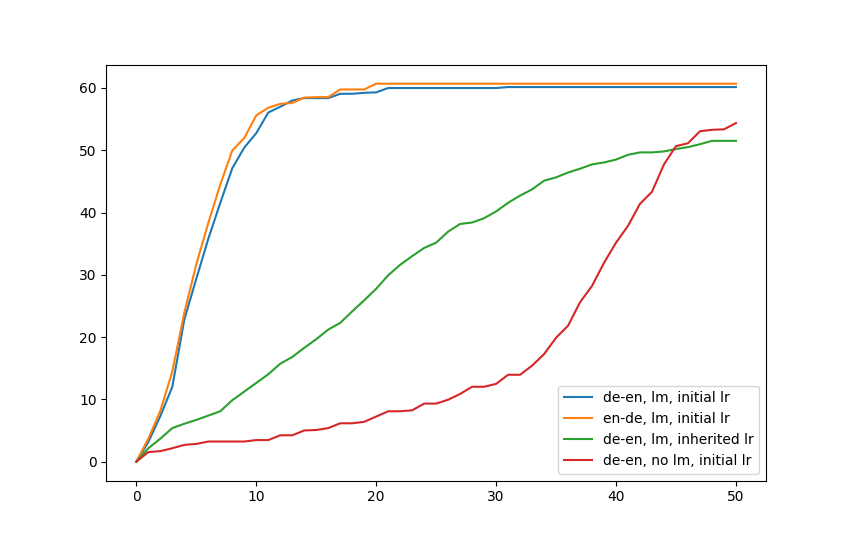
\includegraphics[width=10cm]{corpus}
	\centering
	\caption{Comparison of different experiments}
\end{figure}


\section{Sentence Translation}


\subsection{Overall Results}
\begin{table}[H]
	

	\centering
		\scalebox{0.8}{
		\begin{tabular}{lcccc}
			\toprule
			& De-En & En-De & Fr-En & En-Fr\\
			System   & \textsc{Bleu} [\%] & \textsc{Bleu} [\%] & \textsc{Bleu} [\%] & \textsc{Bleu} [\%]\\
			\midrule
			Word-by-Word   & 11.1 & 6.7 & 10.6 & 7.8\\
			\midrule
			+ LM (5-gram) + tgt w/ high LM score for OOV  & 12.9 & 8.9 & 12.7 & 10.0\\
			+ LM (5-gram) + copy from src for OOV		& 14.5 & 9.9 & 13.6 & 10.9\\
			\midrule
			\hspace{10pt}+ Denoising (RNN)  & 16.2 & 10.6 & 15.8 & 13.3 \\
			\hspace{10pt}+ Denoising (Transformer) & \leavevmode\color{blue}{17.2} & \leavevmode\color{blue}{11.0}& \leavevmode\color{blue}{16.5} & \leavevmode\color{blue}13.9 \\
			\midrule
			\cite{lample2017unsupervised} & 13.3 & 9.6 & 14.3 & 15.1\\
			\cite{artetxe2017unsupervised} & - & - & 15.6 & 15.1\\
			\bottomrule
		\end{tabular}}
	\caption{Translation results on German$\leftrightarrow$English \texttt{newstest2016} and French$\leftrightarrow$English \texttt{newstest2014}}

\end{table}
As demonstrated in Table LM improves wordby-word
baselines consistently in all four tasks, giving at least +3\% BLEU. When our denoising
model is applied on top of it, we have additional
gain around +3\% BLEU. Note that our methods
do not involve any decoding steps to generate
pseudo-parallel training data, but still perform
better than unsupervised MT systems that rely on
repetitive back-translations by up to +3.9\% BLEU.
%above, our unsupervised MT surpass the start-of-the-art unsupervised NMT in almost all cases except English$\rightarrow$French translation. Each sub-model lift the performance respectively. Copy OOV word from source sentences works better than those predicted by language model, because OOV words are usually specific name entities and LM prefers common words rather than rare words. Denoising autoencoder based on Transformer structure outputs better translation than the traditional RNN structure. 


	\begin{table}[!h]
	\centering
	\caption {Word-by-word translation from German to English}
	\begin{tabular}{ccc}
		\hline
		&\textsc{Accuracy} [\%]& \textsc{Bleu} [\%] \\ \hline
		5M & 44.9  & 9.7  \\ \hline
		10M & 51.6 & 10.1 \\ \hline
		50M & 59.4 & 10.8 \\ \hline
		100M &\leavevmode\color{blue}61.2 & \leavevmode\color{blue}11.2 \\ \hline
	\end{tabular}
\end{table}
As in Table 6.9, larger corpus improves the word translation accuracy as well as the word-by-word translation. 

\subsection{BPE vs Word}
Byte pair encoding (BPE)(\cite{sennrich2015neural}) is a simple data compression technique for word segmentation. It allows for the representation of an open vocabulary through a fixed-size vocabulary of variable-character sequences, making it very suitable word segmentation strategy for neural network models. It helps to reduce the vocabulary size and they eliminate the presence of unknown words in the output translation. We use BPE to represent the mapping between languages and compare with word-level cross-lingual embeddings. In BPE algorithm, the vocabulary is updated using an iterative greedy algorithm. Merges in Table 6.7 denotes the pre-defined number of merge operations. 
	\begin{table}[h]

	\centering
	\scalebox{1}{
		\begin{tabular}{lcc}
			\toprule
			\multicolumn{2}{c}{\textbf{Vocabulary}} & \textsc{Bleu} [\%] \\
			\midrule
			& Merges \\
			\cmidrule{2-2}
			\multirow{3}{*}{BPE} & 
			20k & 10.4 \\
			& 50k & 12.5 \\
			& 100k & \leavevmode\color{blue}13.0 \\
			\midrule
			& Cross-lingual training \\
			\cmidrule{2-2}
			\multirow{4}{*}{Word} & 20k & 14.4\\
			& 50k & 14.4\\
			& 100k & \leavevmode\color{blue}14.5\\
			& 200k & 14.4\\
			\bottomrule
		\end{tabular}
	
	}\\
	\caption{Different embedding units and vocabulary size}
\end{table}


%As in Table 6.10, the BPE performs worse than word in this unsupervised learning scenario. It might be difficult to learn the translation relationship between subword units. Also for sentence translation, larger vocabulary size does not improve the performance. In order to balance the efficiency and accuracy we limit the vocabulary size to 50k. To improve the results, LM are exploited here.
We examine how the translation performance varies with different vocabularies of cross-lingual word embedding in Table 6.7. The first three show that BPE embeddings performs worse than word embeddings, especially with smaller vocabulary size. For small BPE tokens (1-3 characters),
the context they meet during the embedding
training is much more various than a complete word, and a direct translation of such small
token to a BPE token of another language would be very ambiguous. For word level embeddings, we compared different vocabulary sizes used for training the
cross-lingual mapping. Surprisingly, cross-lingual word embedding learned only on top 20k words is comparable to that of 200k words in the translation quality. This means that word-by-word translation with crosslingual embedding depends highly on the frequent word mappings, and learning the mapping between rare words does not have a positive effect. 

\subsection{Artificial Noise}

	\begin{table}[H]

	\centering
	\scalebox{1}{
		\begin{tabular}{cccrc}
			\toprule
			$d_\text{per}$ & $p_\text{del}$ & $p_\text{ins}$ & $V_\text{ins}$ & \textsc{Bleu} [\%] \\
			\midrule
			2 & & & & 14.7\\
			3 & & & & \leavevmode\color{blue}{14.9}\\
			5 & & & & 14.9\\
			\midrule
			\multirow{2}{*}{3} & 0.1 & &  & \leavevmode\color{blue}{15.7} \\
			& 0.3 & & & 15.1 \\
			\midrule
			\multirow{4}{*}{3} & \multirow{4}{*}{0.1} & \multirow{4}{*}{0.1} & 10 & 16.8 \\
			& & & 50 & \leavevmode\color{blue}{17.2} \\
			& & & 500 & 16.8 \\
			& & & 5000 & 16.5\\
			\bottomrule
		\end{tabular}
	}

	\label{tab:denoising}
		\caption{Different artificial noises}
\end{table}
To examine the effect of each noise type in denoising
autoencoder, we tuned each parameter of the noise and combined them incrementally as in Table 6.8.  Firstly, for permutations, a significant improvement is achieved from $d_{per}$ = 3, since a local
reordering usually involves a sequence of 3 to 4
words. With $d_{per} le 5$ , it shuffles too many consecutive
words together, yielding no further improvement.
This noise cannot handle long-range reordering, which is usually a swap of words that are far from each other, keeping the words in the
middle as they are. \\
Secondly, we applied the deletion noise with
different values of $p_{del}$. 0.1 gives +0.8\% BLEU, but we immediately see a degradation with a larger value; it is hard to observe more than one one-tomany
translations in each German→English sentence pair.
Finally, we tested several sizes of $V_{ins}$ for the
insertion noise, fixing $p_{ins}$ = 0.1. Increasing $V_{ins}$
is generally not beneficial, since it provides too
much variations in the inserted word, which might
not be related to its neighboring words. Overall,
we observe the best result (+1.5\% BLEU) with
$V_{max} = 50$.



\subsection{Phrase Embedding}

\begin{table}[h]
	\centering
	\begin{tabular}{ccccc  c}
		\hline
		\multicolumn{3}{c}{\multirow{2}{*}{\textbf{Vocabulary}}}                  & No LM & With LM & Denoising \\
		\multicolumn{3}{c}{}                                         &  \textsc{Bleu} [\%]  &  \textsc{Bleu} [\%] & \textsc{Bleu} [\%]   \\ \hline
		Word            & \multicolumn{2}{l}{}              & 11.2 & 14.5  &\leavevmode\color{blue}{ 17.2} \\
		\hline
		\multirow{3}{*}{\cite{mikolov2013distributed} } & \multirow{3}{*}{threshold} & 100  & 11.1 & 13.7  & 15.6 \\ \cline{3-6} 
		&                            & 500  & 11.0 & 13.7  & 16.2 \\ \cline{3-6} 
		&                            & 2000 & 10.7 & 14.0  &16.5 \\ \hline
		Top frequent              & \multicolumn{1}{l}{\text{count}}  & 50k  & \leavevmode\color{blue}12.0 & \leavevmode\color{blue}15.7  & 16.8 \\ \hline
	\end{tabular}
	\caption{Performance of phrase embedding in MT}
\end{table}
With word2vec tool (\cite{mikolov2013distributed}) we detect phrases in the training corpus. We set threshold value to 100, 500, 2000 to make the number of phrases differs. Fewer phrases will be detected as we lift the threshold value. As to our method, we extract only bigrams that in the top 50k frequent bigrams in the training corpus. We learn phrase embedding in an unsupervised manner as normal word embedding. \\
As demonstrates in Table
%?????? not sure if I need to add this corresponding part in unsupervised cross-lingual embedding


%\subsection{Vocabulary Cutoff in Translation}
%\begin{table}[h]
%	\parbox{.5\linewidth}{
%		\centering
%		\caption{Word embedding vocabulary cut-off}
%		\begin{tabular}{c c c c } 
%			\hline
%			\textsc{Bleu} [\%]	& 20k & 50k & 100k \\
%			\hline
%			50k &	11.1  & \leavevmode\color{blue}11.3 & 11.2  \\ 
%			\hline
%			100k&	11.2  & 11.2 & 11.1 \\ 			
%			\hline
%			150k&	10.9 & 10.9 & - \\
%			\hline
%		\end{tabular}
%		
%	}
%	\hfill
%	\parbox{.5\linewidth}{
%		\centering
%		\caption{Phrase embedding vocabulary cut-off}
%		\begin{tabular}{c c c c } 
%			\hline
%			\textsc{Bleu} [\%]	& 50k & 100k & 150k \\
%			\hline
%			50k &	11.3  & - & -  \\ 
%			\hline
%			100k&	11.9  & 11.9 & - \\ 			
%			\hline
%			150k&	\leavevmode\color{blue}12.0 & 11.9 & 11.9 \\
%			\hline
%			200k & 12.0 & - & - \\
%			\hline
%		\end{tabular}
%		
%	}
%\end{table}
